\begin{frame}{Blue Gene/P}
    \begin{quote}\large \centering
    The easiest way to make software scalable \\
    is to make it sequentially inefficient. \\
    (Gropp 1999)
  \end{quote}

  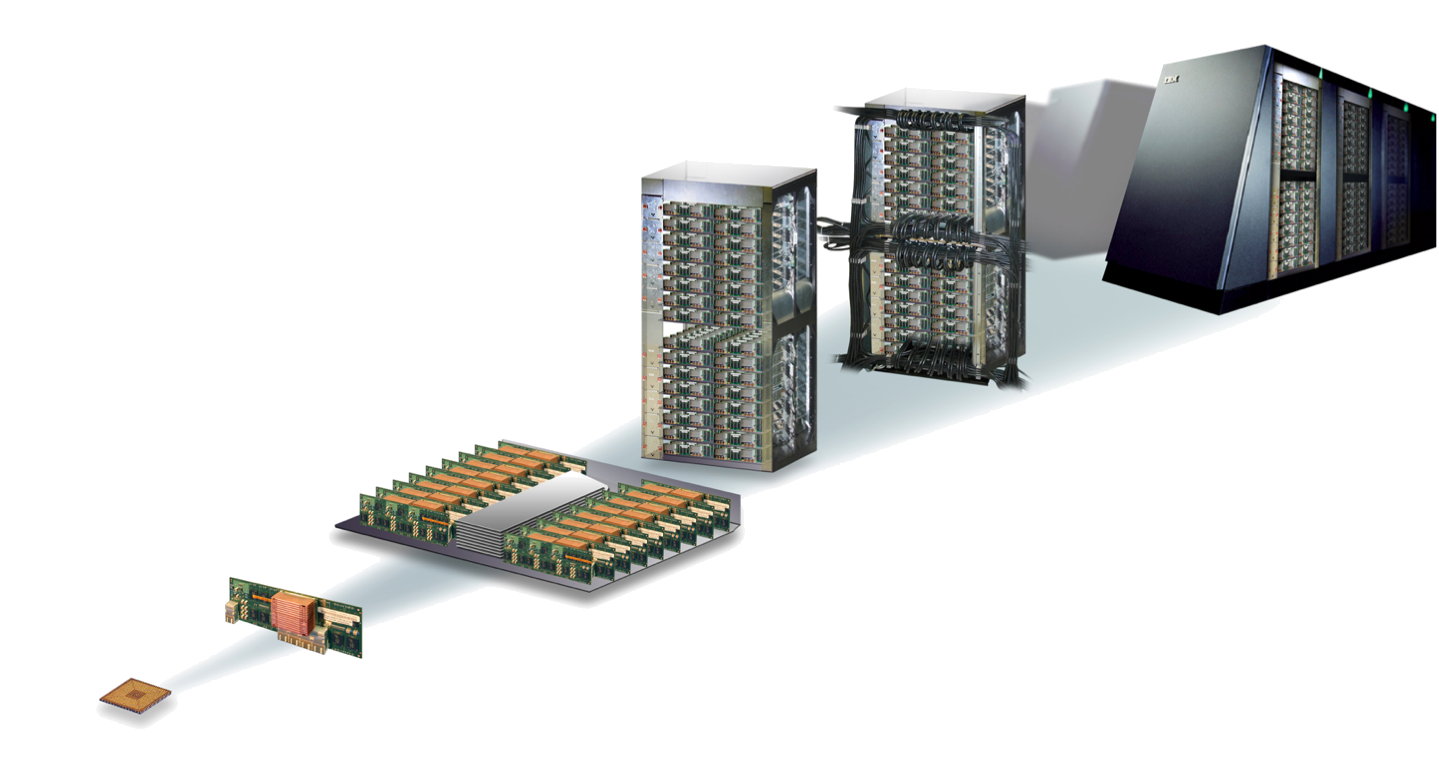
\includegraphics[width=\textwidth]{figures/BlueGenePRacks}
\end{frame}
\begin{frame}{Blue Gene/P}
  \begin{columns}
    \begin{column}{0.6\textwidth}
      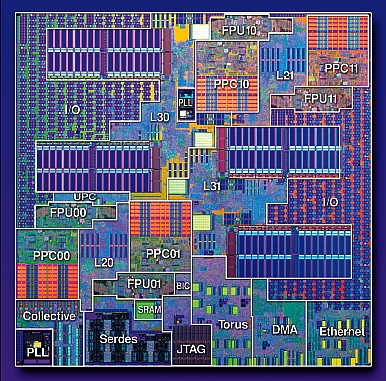
\includegraphics[width=\textwidth]{figures/BlueGenePDie}
    \end{column}
    \begin{column}{0.4\textwidth}
      \begin{itemize}
      \item 4 cores @ 850 Mhz
      \item 32 16-bytes FP registers
      \item 1 packed FMA per cycle, latency 5
      \item 0.5 load per cycle, latency 4
      \item 3 memory requests in-flight
      \item write-through cache, FIFO eviction policy
      \item up to 5 memory streams
      \end{itemize}
    \end{column}
  \end{columns}
\end{frame}
